\documentclass{article}
\usepackage[UKenglish]{babel}

\usepackage{graphicx}
\usepackage{booktabs}
\usepackage{tabularX}
\usepackage{multirow}
\usepackage{amsmath}
\usepackage{natbib}
\usepackage{color}
\usepackage{adjustbox}

\usepackage[paperwidth=174mm, paperheight=62mm, margin=0cm]{geometry}
%\renewcommand{\familydefault}{\sfdefault}
\usepackage{fontspec}
\setmainfont{Arial}
\setlength\parindent{0pt}

\begin{document}
\hspace{-0.5em}
\begin{tabular}{l@{\hspace{4mm}}l@{\hspace{4mm}}l}
  \large{A} &\large{B} &  \large{C} \\
  \includegraphics[width=56mm]{Figure6aM.pdf}&\includegraphics[width=56mm]{Figure6bM.pdf}&
  \hspace{-1mm}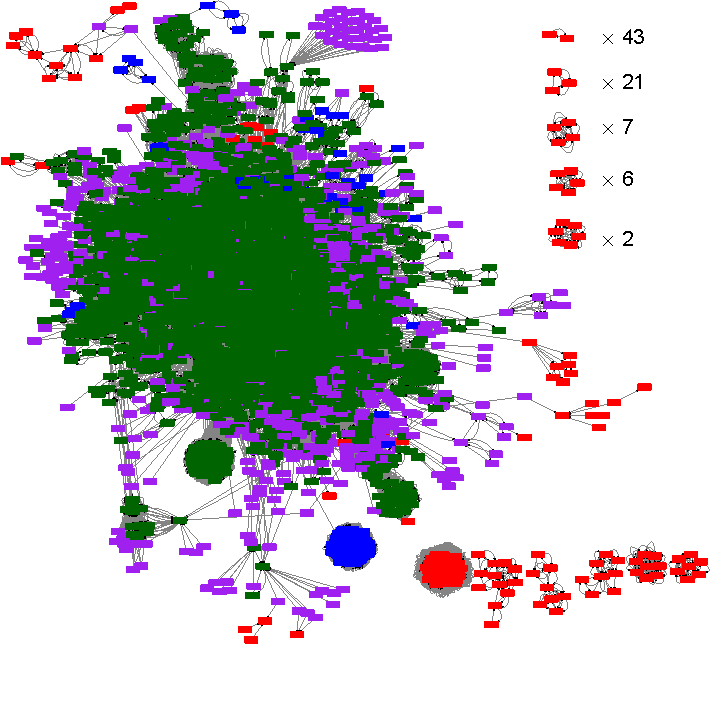
\includegraphics[width=53mm]{Figure6cColour.pdf}
\end{tabular}
\end{document}

